%!TEX root = Report.tex

\subsection{Graphical user interface}
\begin{figure}[ht!]
  \centering
    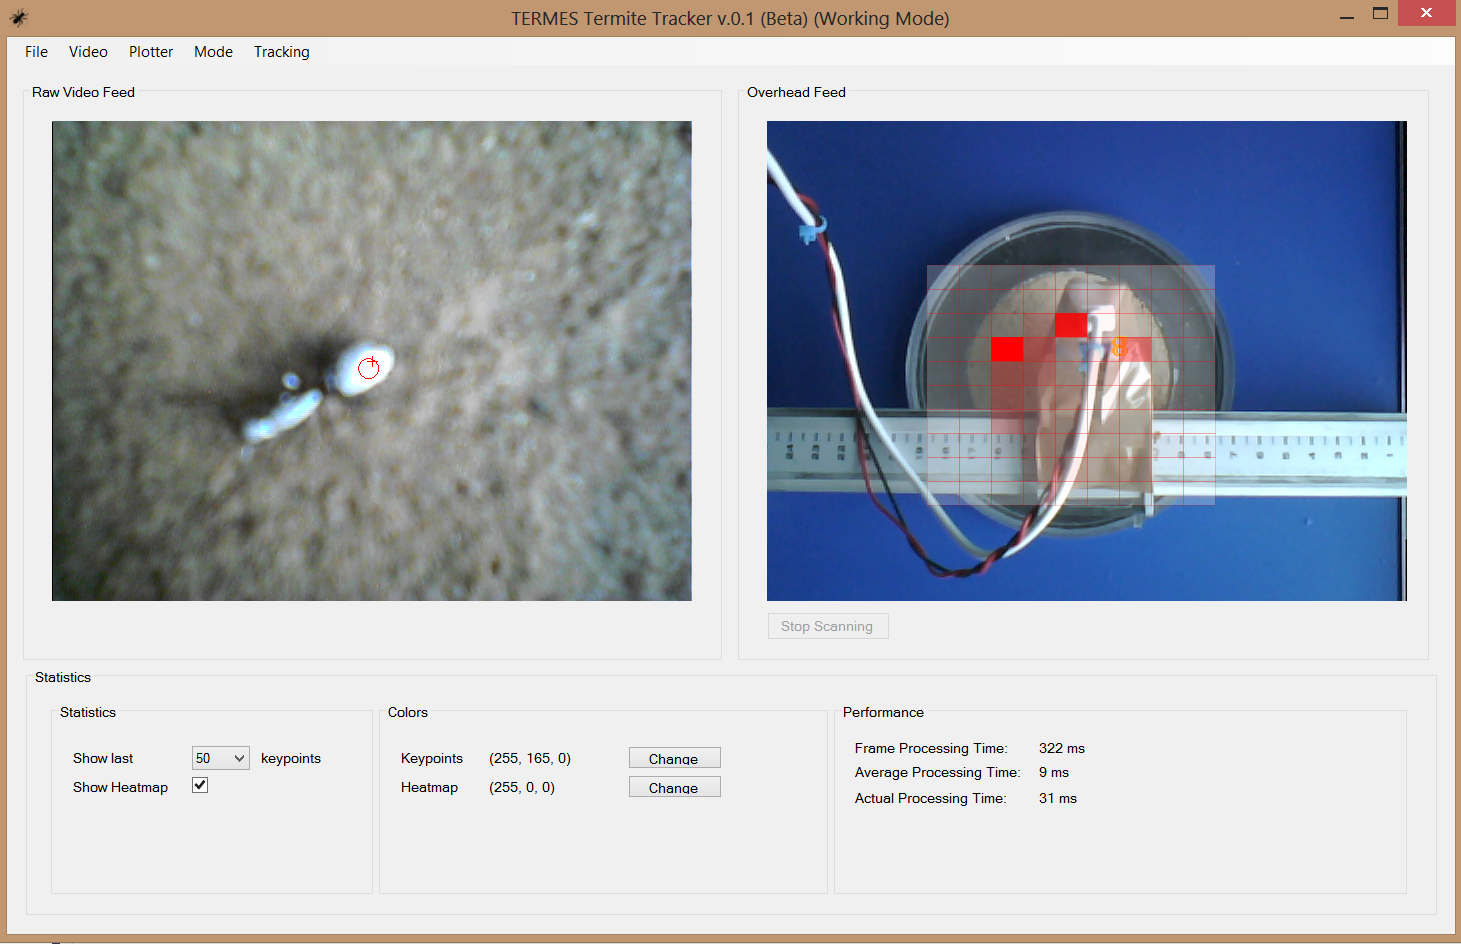
\includegraphics[scale=0.25]{img/HeatmapGUI}
  \caption{GUI in tracking mode with heatmap statistic.}
  \label{fig:gui_heat}
\end{figure}

\subsection{Graphical user interface}
\begin{figure}[ht!]
  \centering
    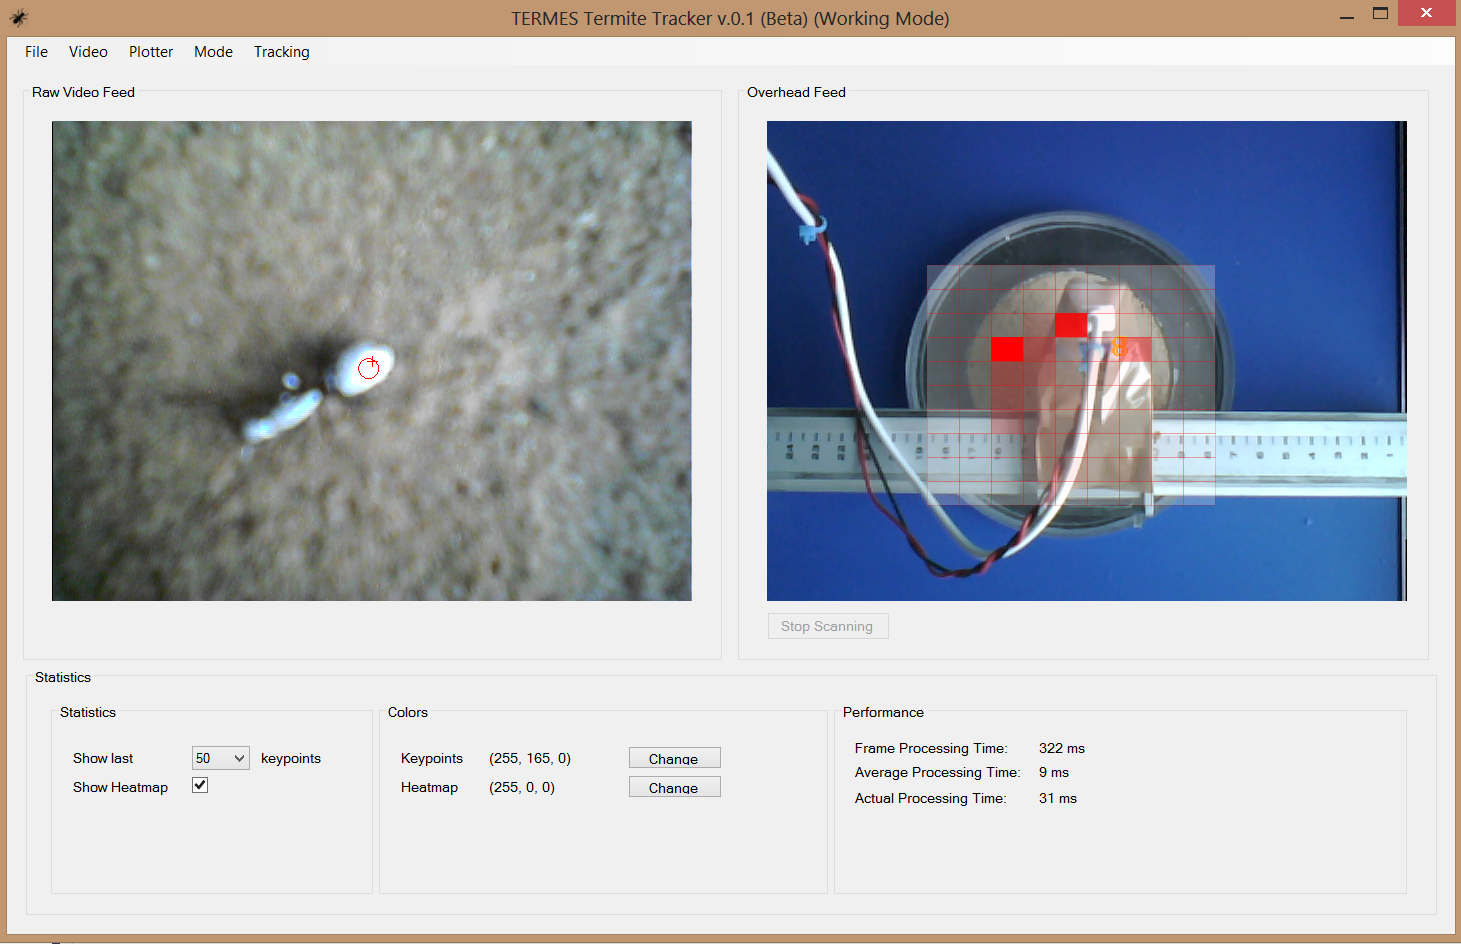
\includegraphics[scale=0.25]{img/HeatmapGUI}
  \caption{GUI in tracking mode with heatmap statistic.}
  \label{fig:gui_thresh}
\end{figure}

In order to use the system to track ants, we needed a user interface. The requirements for the user interface are the following:

\begin{itemize}
  \item{It should be able to show the camera feed from both the mobile and the overhead camera}.
  \item{It should be able to calibrate the system before initiating the tracking procedure}.
  \item{It should provide a way to gather statistics during the process of tracking}.
  \item{It should provide a set of controls to manipulate the plotter manually}.
\end{itemize}

\todo{Indsæt reference til JNI}

We chose to implement the GUI in Windows Forms using C\# because it was a requirement that all software would run at least on Windows but preferably on other platforms as well. We experimented with a Swing GUI in Java, however we experienced problems with calling into C++ code on Windows using Java Native Interface (JNI) so we chose to switch to C\# in order to save time. \\

Furthermore, it is easy to integrate C++ code with .NET as no libraries like JNI are needed. All C++ logic is published as a DLL with an interface represented in the GUI. The GUI is shown in Figure \ref{fig:gui_heat}. \\

As seen from the figure, the GUI consists of a horizontal menu bar in the top, a video feed for the mobile camera on the left and a video feed for the overhead camera on the right. In the bottom, a panel is placed to display various statistics about the tracking process and the current performance of the system such as processing time, etc. \\

The GUI provides two modes - one for calibration and one for tracking. Switching between tracking and calibration mode is done through the \texttt{Mode} menu point in the top menu. When in calibration mode, the right camera feed will switch and show a thresholded version of the mobile view instead. Likewise, the lower panel will reveal a slider for setting the threshold value. Thresholding is one of the key techniques behind the tracking and the quality varies with the light and general surroundings of the camera, so it is important to be able to adjust it between and during sessions. The result of changing the threshold value is visible in real time in the right camera feed, thus, it is possible to stay in calibration mode while tracking. \\

Ideally, the camera should be located above the ant when setting the threshold value, as we are essentially telling the system how to identify the ant. To do this, open the manual steering panel by selecting \texttt{Manual Steering} from the plotter menu in the top bar. This panel provides controls similar to the arrow keys on a keyboard for manipulating the plotter. Using the keys and the camera feeds and provided that the ant is not moving too quickly, it is possible to adjust the plotter so the camera is located above the ant. This process might require leaving the ant in the freezer for a couple of minutes beforehand. By default, the plotter will move 5 units each time a button is clicked. This number can be adjusted for each axis individually by setting the textfields in the right side of the window. Alternatively, use the controls in the top of the window to go directly to a specific coordinate.\todo{insæt referencer til billeder} \\

When the camera is in place, return to the slider and adjust it until the ant is the largest white blob on screen. Ideally, the ant should be the only white object, but the system will look for the largest object so a reasonable amount of minor objects or noise are allowed to be visible as well. \\

When thresholding is in place, tracking is started by choosing \texttt{Start} under \texttt{Tracking} in the top menu. The camera will track the ant and show statistics in the panel until the user presses \texttt{Stop} or the ant is lost in the picture. In either case, the process can be repeated to start tracking again.

%What was the reqs for the GUI?
%How did we want it to look?
%What tasks do we expect the users to do (normal work flow)?
%Are we satisfied with the GUI (eval)?
%JNI skulle være cross platform men fungerede ikke med OpenCV.
%(nævn at det ville have været nice at have det cross platform)
%Vi har ikke noget der finder myren til at starte med. Hvordan kunne dette gøres?

% \begin{figure}[!ht]
%     \centering
%     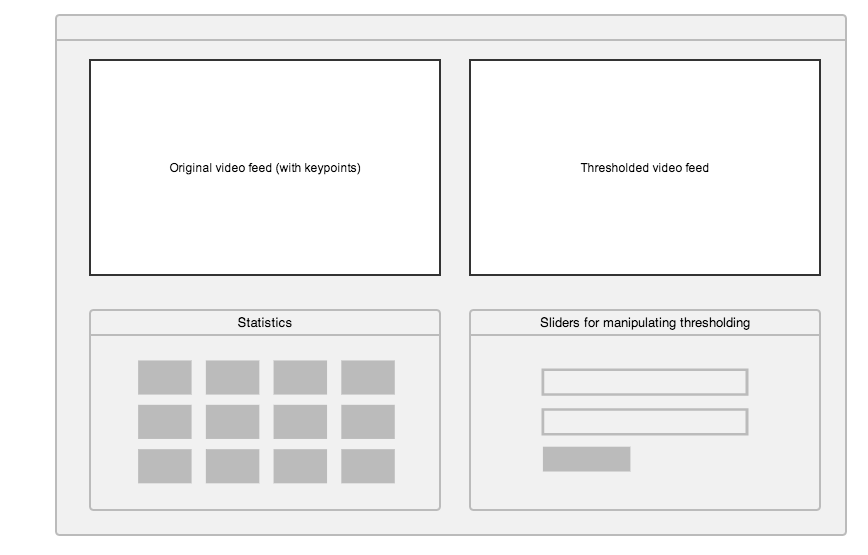
\includegraphics[scale = 0.3]{img/termes_gui.png}
%     \caption{Initial GUI draft}
%     \label{fig:gui}
% \end{figure}

\subsubsection{Statistics} \mbox{}\par
One of the requirements to the GUI is that it is able to present relevant statistics to the user in a natural way. We chose to focus on the statistics that have a somewhat graphical presentation, we decided to implement the following statistics:

\begin{itemize}
  \item{The route of the ant.}
  \item{A heatmap.}
  \item{Performance indicators.}
\end{itemize}

Since the purpose of the software is to enable users to track ants, it seems natural to provide a graphical view of the route. In the current version, when tracking is enabled, the user can choose to display the last $x$ locations of the ant where $x$ can be adjusted from the drop down menu in the statistics panel. Whenever a number greater than zero is chosen, the locations appear as small circles in the overhead frame.
The color of the circles can be adjusted in the GUI as well. \\	

The second statistic is a heatmap. The heatmap is visualized as a 2D array of rectangles drawn in the overhead frame. While the route statistic provides location information, the heatmap provides this information over time. When tracking is started, the program will capture the location of the ant, find the encapsulating rectangle and keep incrementing the intensity of the color in that rectangle until the ant enters a neighbouring rectangle. After a few minutes of tracking, the color intensities of the heatmap will reveal the preferred location of the ant during those minutes. \\

The three performance indicators that we provide are located in the lower statistics panel to the right. These indicate the overall performance of the system in terms of frame processing time, image processing time and average image processing time in milliseconds. Frame processing time indicates how much time is spent on each frame in total including image processing, updating statistics etc. Image processing time covers time spent exclusively on image processing. This includes thresholding, blob extraction, copying frames to and from the GPU etc. Average image processing is simply an average of time spent on image processing of frames. We believe these last statistics are useful especially for troubleshooting. \\

In order to be able to keep the results gathered from tracking, the program saves all statistics in a log file which is placed next to the programs executable file when the user stops the tracking in the GUI.

%What statistics do we extract?
%How do the users do this?
%How are they produced?
%Can they be improved (future work)?
